\documentclass{article}

\usepackage[%
    left=0.5in,%
    right=0.5in,%
    top=0.5in,%
    bottom=0.5in,%
]{geometry}%
\usepackage{minitoc}
\usepackage{multicol}
\usepackage{graphicx}
\usepackage{fixltx2e}
\usepackage{listings}
\usepackage{color}
\usepackage{hyperref}
    \hypersetup{ colorlinks = true, linkcolor = blue }
\usepackage{blindtext}
\definecolor{lightgray}{gray}{0.9}
\graphicspath{ {./} }

\newcommand{\inlinecode}[2]{\colorbox{lightgray}{\lstinline
[language=#1]$#2$}}
\newcommand{\worddef}[1]{\hyperref[sec:reference]{\textit{#1}}}

\begin{document}

\tableofcontents

\newpage

\section{Logical	Data	Storage	on	Android}

\begin{flushleft}
File-based abstractions
\begin{itemize}
  \item Shared Preferences: Simple key value pairs
  \item File-based storage:
  \begin{itemize}
    \item Internal Data Storage: Soldered RAM. Internal APK resources, temporary files
    \item External Data Storage: SD Card. Large media files
  \end{itemize}
  \item SQLite Database: Structured data, small binary files
\end{itemize}
Network sync adapters:
\begin{itemize}
  \item Shared contact lists, backups
  \item Synchronising local and remote files
\end{itemize}
\end{flushleft}

\section{Internal File Storage}

\begin{flushleft}
Internal	Data	storage	is	private	to	the	
\begin{itemize}
  \item Other apps (and the user) cannot access it: Kernel enforced user permissions
  \item Removed	on	uninstall: so sensitive data cannot be obtained
  \item Data is stored in files:
  \begin{itemize}
    \item /data/data/com.example.martinstorage/files/
    \item openRawResource: Can be used to read our own packaged resources
  \end{itemize}
\end{itemize}
Android provides a standard place to store (small) cache files
\begin{itemize}
  \item FingerPainterView
  \item /data/data/com.example.martinstorage/cache
  \item getCacheDir() to get a File for the directory
  \item We should still manage the files ourselves
  \begin{itemize}
    \item May be deleted when internal storage becomes full / contested
    \item Will be deleted when the application is uninstalled 
    \item A “well behaved” application will delete them when no longer in use. Recommended to use less than 1MB
  \end{itemize}
\end{itemize}
\end{flushleft}

\subsection{Shared Preferences}

\begin{itemize}
  \item In internal Storage , stored on a per-application basis 
  \item I.e. all components in an application may access the same Shared Preferences 
  \item But should not be used for data transfer (instead of Intents, Binder etc) 
  \item Primitive data in key-value pairs. Primitives: strings, integers etc. Not Bundles 
  \item Can have multiple preference files per application
\end{itemize}

\section{External storage}
\begin{flushleft}
Every	Android	device	provides	externally-accessible	storage,	e.g.	SD	card
\begin{itemize}
  \item Even those phones without an SD card. They have a logical representation of “external” storage 
  \item Single storage device partitioned into internal / external. This is because all Android devices must conform to the Android API in order to be Android devices 
  \item “Private” application files. Internal Storage on the External partition (Else permissions cant be overriden with other device) 
  \item “Public” general files
  \begin{itemize}
    \item World readable 
    \item Other applications can read and modify these files 
    \item Each “user” has their own virtual SD card
  \end{itemize}
\end{itemize}
Can be mounted externally (and/or disconnected). Before accessing files need to check the state of external storage. It may not be there, or mounted by something else
\end{flushleft}

\subsection{Using external storage}

\begin{itemize}
  \item Should check state with \verb|Environment.getExternalStorageState()|. It is a separate file system, potentially removable. \verb|Environment.MEDIA_MOUNTED|, \verb|Environment.MEDIA_MOUNTED_READ_ONLY|.
  \item Use \texttt{getExternalStoragePublicDirectory(String type)} to obtain a File for the directory
  \begin{itemize}
    \item Pass a type to obtain a sub-directory for that type 
    \item Used to enable the Media scanner to categorize material 
    \item Use File object returned to createNewFile() 
    \item Scoped Directory access 
    \item “With each new release, developers have been provided with new and updated APIs to work with”
  \end{itemize}
  \item \verb|getExternalFilesDir()|
  \item Provides private external storage 
  \item /sdcard/Android/data/com.example.pszmdf.fingerpainter/
\end{itemize}

\section{Android Databases}

\begin{itemize}
  \item Often the data we are storing is logically structured
  \begin{itemize}
    \item Need to query it based on that structure 
    \item Could store this in a file and write our own routines to access it 
    \item Obb virtual file system 
    \item StorageManager (wrapper for MountService system service) 
    \item Opaque Binary Blobs 
    \item Normally, we’d use a database to store it 
    \item E.g. An address book, music library
  \end{itemize}
  \item Android provides local database support
  \begin{itemize}
    \item Complete with the ability to run full SQL queries. Each app’s databases are local to it 
    \item Database.db stored in Internal Storage (SQLite)
  \end{itemize}
\end{itemize}

\subsection{Android and SQLite}

\begin{itemize}
  \item Wrapped up in two main classes
  \begin{itemize}
    \item Database represented by SQLiteDatabase 
    \item Lets us run SQL queries on the database 
    \item SQLiteOpenHelper: Supports the Application lifecycle. \verb|onCreate()|. Create the database the first time the application is opened. \verb|onUpgrade(int oldVersion, int newVersion|. Changing the version number affords drop and recreation of the database
  \end{itemize}
  \item Create an instance of our SQLiteOpenHelper subclass 
  \item Obtain reference to SQLiteDatabase using: \verb|getReadableDatabase(), getWriteableDatabase()| Both return the same object, unless memory is low and can only open the DB readonly
\end{itemize}

\subsection{Cursors}

\begin{itemize}
  \item Provides random access to results of a query
  \item Enable us to step over all the rows returned by a query \verb|moveToFirst(), moveToNext()| 
  \item \verb|getString(columnIndex), getInt(columnIndex)|. Where column index is index of projection result 
  \item Has a \verb|close()| method to close the query when finished. Shouldn’t wait for it to be garbage collected 
  \item IPC implications. Can we pass a cursor to another process? (component number 3)
\end{itemize}

\subsection{Data Driven Views}

\begin{flushleft}
“Connect” a cursor to a CursorAdapter and ListView
\begin{itemize}
  \item SimpleCursorAdapter(...Cursor...) 
  \item Map the projection to a View layout for a single item, populate a list of views 
  \item Link resource IDs to projection columns. Requires each row to have an \verb|_id| field 
  \item Automatically generates a View for each row of the cursor
\end{itemize}
RecyclerView
\begin{itemize}
  \item Optimised, flexible version of the above 
  \item Only creates Views for visible data 
  \item As the user scrolls, or more data is added 
  \item Create new Views as appropriate. Re-bind old Views to new data 
  \item Programmatically describe how to create View from data
\end{itemize}
\end{flushleft}

\subsection{CursorLoader}

\begin{flushleft}
  \item A query may last some time. Database may be large, may be in a different process. We Don’t want to block the main UI thread
  \item \textbf{CursorLoader}: Populates views asynchronously, Auto Updating, Monitors for notification that content has changed
\end{flushleft}

\subsection{Database Abstraction}

\begin{flushleft}
Good software architecture. Separation of data model from presentation / views. Abstraction of database architecture:
\begin{itemize}
  \item Easier to update storage code 
  \item Expose column indices as static class variables: \verb|c.getInt(0) -> c.getInt(DBHelper.NAME)|
  \item Helper methods keep database internals from “leaking” into other classes. Return a Collection of results rather than a Cursor. Use Cursor internally in DBHelper class 
  \item SQL injection: Sanitise user input 
  \item Important when thinking about the logical next step – exposing data to other applications via a Component. Appropriate database schema
\end{itemize}
\end{flushleft}

\section{Sharing data}

\subsection{Content	Provider}
\begin{flushleft}
Access to data is restricted to the app that owns it
\begin{itemize}
  \item Database is usually located in internal app-specific storage (Inaccessible by other applications)
  \item If we want other apps to access our data, or we want to access other apps’ data, or we want to be notified when data has changed
\end{itemize}
Provide or make use of a Content Provider
\begin{itemize}
  \item Application component number 3 
  \item Exposes data / content to other applications in a structured manner 
  \item Fundamentally IPC via Binder (again) + ashmem with a well defined (database-like) interface
\end{itemize}
\end{flushleft}

\subsection{System Content Providers}

\begin{flushleft}
Content Providers manage data for:
\begin{itemize}
  \item Browser: Bookmarks, history
  \item Call log: Telephone usage
  \item Contacts: Contact data, WhatsApp?
  \item Media: Media metadata database
  \item UserDictionary: Database for predictive spelling
  \item And other common mobile capabilities
\end{itemize}
Good practice even when making data available only within the application
\begin{itemize}
  \item Either create a new one (by sub-classing ContentProvider) 
  \item Or add / query data via an existing / native Content Provider
\end{itemize}
Assuming that spawning an Activity via Intent is not sufficient
\begin{itemize}
  \item Querying complex data 
  \item Task flow 
  \item Requiring close coupling of application to data. c.f. Binding to Services
\end{itemize}
\end{flushleft}

\subsection{Data Model}

\begin{flushleft}
Content Providers implement a specific data model. Very similar to a relational database table:
\begin{itemize}
  \item A collection of records 
  \item Support for reading and writing 
  \item Support typical database operations: CRUD
\end{itemize}
Records are stored in rows, with each column providing different data fields
\begin{itemize}
  \item Each record has a numeric id (in the field \verb!_ID!) that uniquely identifies it
\end{itemize}
Tables exposed via URI
\begin{itemize}
  \item Abstraction again, can be close to or distant from underlying storage 
  \item Most of the “work” is specifying the abstraction / linkage
\end{itemize}
\end{flushleft}

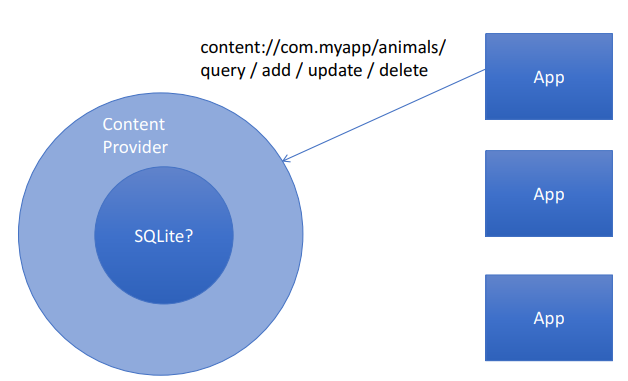
\includegraphics[scale=0.5]{data_model.png}

\subsection{Querying a Content Provider}

\begin{flushleft}
\textbf{ContentResolver}
\begin{itemize}
  \item Manages and supports Content Provider access 
  \item How to service a request for content (Similar to ServiceManager) 
  \item Enables Content Providers to be used across multiple applications (Provides additional services such as change notification)
  \item Can observe a Content Provider to be informed of real-time modifications
  \begin{itemize}
    \item A new MP3 has been added to the library 
    \item ContentObserver
  \end{itemize}
\end{itemize}
\textbf{Content Providers identify data sets through URIs}
\begin{itemize}
  \item \textbf{content://authority/path/id} 
  \item \textbf{content}: Data managed by a Content Provider 
  \item \textbf{authority}: ID for the Content Provider (i.e. fully qualified class name, com.example.martindata) 
  \item \textbf{path}: 0 or more segments indicating the subset of data to be requested e.g. table name, or something more readable / abstracted. RESTful resource philosophy 
  \item \textbf{id}: Specific record (row) being accessed
\end{itemize}
\end{flushleft}

\pagebreak

\subsection{Querying a Content Provider}
  
\begin{flushleft}
URI for searching Contacts. \verb|ContactsContract.Contacts.CONTENT_URI = "content://com.android.contacts/contacts/"|
\verb|ContentResolver.query(...)|:
\begin{itemize}
  \item Returns a Cursor instance for accessing results 
  \item \textit{Cursor} is a pointer to a \textit{CursorWindow} 
  \item A read-only reference to shared memory allocated by ashmem, retrieved via Binder 
  \item Has to be closed and max CursorWindow size is 2Mb. (Because it's inside shared memory)
  \item \verb|Cursor query(Uri uri, String[] projection, String selection, String[] selectionArgs, String sortOrder)|
\end{itemize}
\end{flushleft}

\subsubsection{Accessing content}

\begin{flushleft}
To access / modify Contacts, requires a Permission
\begin{itemize}
  \item \verb|android.permission.READ_CONTACTS| 
  \item \verb|android.permission.WRITE_CONTACTS|
\end{itemize}
Contacts has three components
\begin{itemize}
  \item Data: Rows (mime-typed) that can hold personal information
  \item RawContacts: A contact for a given person from a given system. Gmail contact, Facebook contact etc, associated with Data entries
  \item Contacts: Aggregated RawContacts, single view of a “person”
\end{itemize}
\end{flushleft}

\subsection{Modifying a Content Provider}

\begin{flushleft}
Done by using \texttt{update} function. We pass \textbf{Uri} and \textbf{ContentValues}, which is key value pairs, where key is name of the column.
\end{flushleft}

\subsection{Creating a Content Provider}

\begin{flushleft}
Implement a storage system for the data:
\begin{itemize}
  \item Structured data / SQLite (Values, binary blobs up to 64k, database)
  \item Large binary blobs (Files)
  \item Photos / media manager
\end{itemize}
Implement a ContentProvider
\begin{itemize}
  \item \texttt{query, add, update, insert} etc 
  \item \texttt{onCreate }
  \item \texttt{getType}. What type of data are we providing? Single item, multiple items, mime types 
  \item ParcelFileDescripter \texttt{openFile()}
\end{itemize}
Tell Android we are a provider. Declare in the AndroidManifest \textbf{android:multiprocess}. Don't use this, it is some old cruft.
\end{flushleft}

\section{Contract}

\begin{itemize}
  \item Defines metadata pertaining to the provider
  \item Constant definitions that are exposed to developers via a compiled .jar file
  \begin{itemize}
    \item Authority (Which app is responsible for this data)
    \item URI schema
    \item Meta-data types 
    \item “Column” names 
    \item Abstraction of database architecture
  \end{itemize}
\end{itemize}

\section{URI Matching}

\begin{flushleft}
All of these methods take a URI as the first parameter
\begin{itemize}
  \item (except for onCreate) 
  \item The object will need to parse it to some extent to know what to return, insert or update
\end{itemize}
\verb|android.content.UriMatcher|: Provides mapping between abstraction of contract class to concrete db implementation
\end{flushleft}

\pagebreak
\section*{Reference section} \label{sec:reference}
\begin{description}
	\item[placeholder] \hfill \\
\end{description}
\end{document}
